\subsection{funktionale und nichtfunktionale Anforderungen}
\label{sec:Kap-6.2.2}

Eine andere Form von Kategorisierung unterscheidet zwischen funktionalen und nichtfunktionalen Anforderungen. Diese Kategorisierung ist prinzipiell unabhängig von der zwischen Nutzer- und Systemanforderungen. So könnte man sowohl in funktionale Nutzeranforderungen und funktionale Systemanforderungen als auch in nichtfunktionale Nutzer- und Systemanforderungen trennen. Üblicherweise wird die so erzeugte Aufteilung in \textbf{vier} Kategorien aber weder in der Literatur explizit thematisiert, noch ist sie in der Praxis besonders bedeutsam. Je nach Kontext steht \textbf{entweder} die Trennung in Nutzer- und Systemanforderungen \textbf{oder} die Trennung in funktionale und nichtfunktionale Anforderungen im Vordergrund.

%hier gehört Abbildung "fig:funktionale_nichtfunktionale_anforderungen" eigentlich hin
\begin{figure}[h!]
	\begin{addmargin*}[0cm]{-\marginparwidth}
	\begin{addmargin*}[0cm]{-\marginparsep}
		\centering
		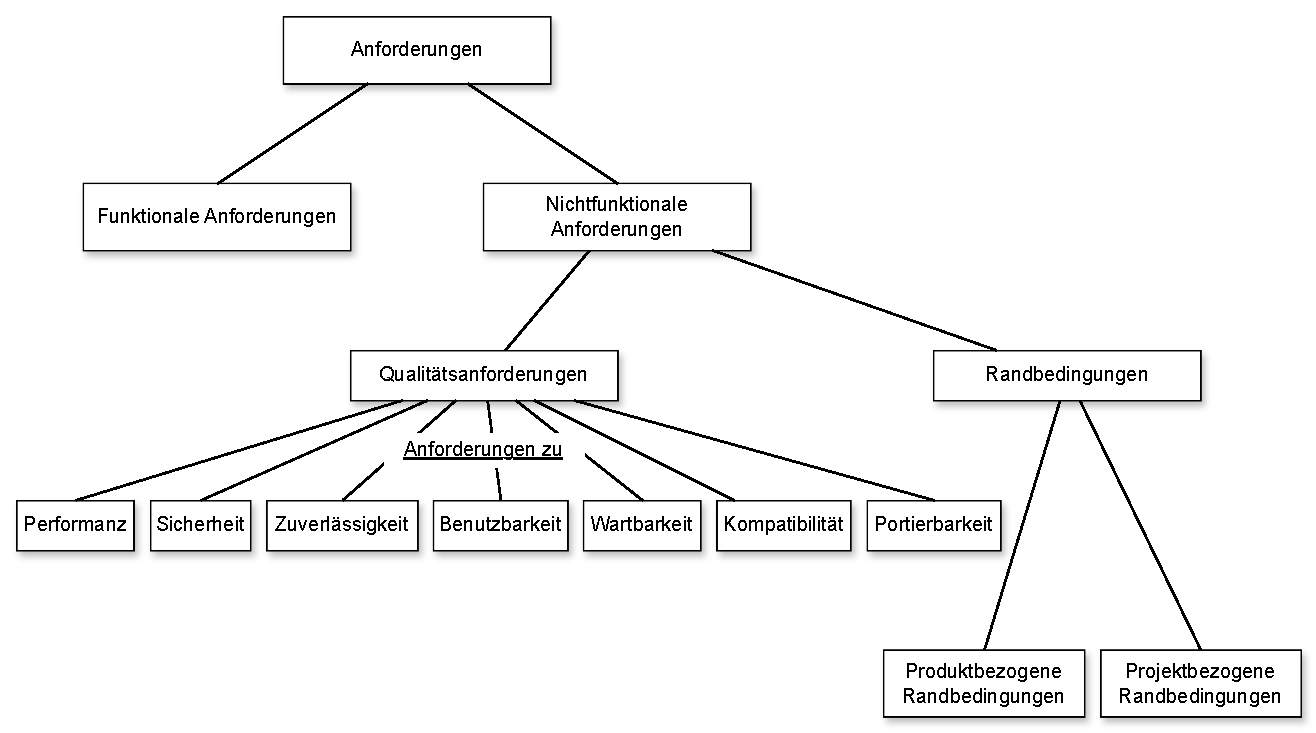
\includegraphics[scale=0.79]{Bilder/Kapitel-6/funktional.pdf}
		\caption{Funktionale und nichtfunktionale Anforderungen}
		\label{fig:funktionale_nichtfunktionale_anforderungen}
	\end{addmargin*}
	\end{addmargin*}
\end{figure}

Abbildung~\ref{fig:funktionale_nichtfunktionale_anforderungen} zeigt die Unterscheidung in funktionale und nichtfunktionale Anforderungen sowie die weitere Untergliederung der nichtfunktionalen Anforderungen. Man kann auch die funktionalen Anforderungen weiter untergliedern. In der Regel sind funktionale Anforderungen aber -- im Gegensatz zu großen Teilen der nichtfunktionalen Anforderungen -- so stark abhängig vom zu entwickelnden Softwareprodukt und dessen zu erwartenden Nutzergruppen, dass jede Form von allgemeiner Kategorisierung für den konkreten Softwareentwicklungsprozess wenig hilfreich ist.

\minisec{Funktionale Anforderungen}

Die funktionalen Anforderungen ergeben sich aus den Tätigkeiten, die Nutzer mit Hilfe des Softwareprodukts durchführen möchten. Sie beschreiben, welche Funktionalitäten (teilweise auch eingedeutscht Features genannt) das Softwareprodukt oder eines seiner Module bereitstellen soll, damit das Produkt von seinen Nutzergruppen sinnvoll eingesetzt werden kann. Funktionale Anforderungen beziehen sich somit auf das gewünschte Verhalten der Software. Sie können in sehr unterschiedlicher Form und auf unterschiedlichen Abstraktionsebenen auftreten. Funktionale Anforderungen sind zum Beispiel 

\begin{itemize}
	\item Vorgaben, welche Ausgabeparameter eine Funktion der Software bei gegebenen Eingabeparametern produzieren soll
	\item Beschreibungen, aus welchen Buttons und Menüeinträgen Benutzeroberflächen bestehen sollen
	\item Vorgaben, zu welchen externen Systemen Schnittstellen existieren müssen
\end{itemize}

Funktionale Anforderungen treten aber sehr häufig auch in der Form von Beschreibungen von Geschäftsprozessen und Anwendungsfällen auf, die durch die Software unterstützt oder durchgeführt werden sollen. Zudem kann über funktionale Anforderungen auch explizit spezifiziert werden, was die Software \textbf{nicht} tun soll.

\minisec{Nichtfunktionale Anforderungen}

Während funktionale Anforderungen festlegen, was das Softwareprodukt leisten können soll, bestimmen die nichtfunktionalen Anforderungen, in welcher Ausprägung, in welcher Qualität und unter welchen Umständen diese Leistungen erbracht werden sollen.

\vspace{\baselineskip} %%% für Druck

\sttpseitenrandzitat{"`Vereinfacht ausgedrückt, legen funktionale Anforderungen fest, was das Softwareprodukt tun soll, während die nichtfunktionalen Anforderungen spezifizieren, wie es arbeiten soll."'}{\cite[109]{bal09}}

\vspace{\baselineskip} %%% für Druck

Nichtfunktionale Anforderungen spezifizieren die Eigenschaften des Gesamtsystems oder schränken diese ein. In die Kategorie der nichtfunktionalen Anforderungen gehören damit Anforderungen, die übergreifende Eigenschaften, Leistungsmerkmale oder Restriktionen des Softwareprodukts betreffen, die nicht in \textbf{direktem} Zusammenhang zu einzelnen Funktionalitäten des Produkts stehen. Im Gegensatz zu den funktionalen Anforderungen, die sich meist einer oder wenigen Komponenten zuordnen lassen, kann die Umsetzung einer nichtfunktionalen Anforderung über viele verschiedene Komponenten des Softwareprodukts verteilt sein. Auch deswegen beeinflussen nichtfunktionale Anforderungen die zukünftige Architektur des Softwareprodukts in erheblichem Maße.

Nichtfunktionale Anforderungen werden heute meistens noch weiter unterteilt in die beiden Kategorien Qualitätsanforderungen und Randbedingungen. Die Randbedingungen nehmen dabei eine gewisse Sonderstellung innerhalb der nichtfunktionalen Anforderungen ein (\su). In mancher Literatur werden sie daher gar nicht den nichtfunktionalen Anforderungen zugeordnet, sondern bilden eine dritte Kategorie von Anforderungen neben den funktionalen und den nichtfunktionalen Anforderungen.

\minisec{Qualitätsanforderungen}

Die Qualitätsanforderungen definieren, welche Qualitätskriterien das Software-
\linebreak %%% für Druck
produkt erfüllen muss. Hier kann man sich an standardisierten Kategorisierungen orientieren und auf dieser Basis die Qualitätsanforderungen für das eigene Softwareprodukt festlegen. Eine solche standardisierte Kategorisierung ist die ISO-Norm 25010:2011 \cite{iso11}. Zu den dort unterschiedenen Kategorien von Qualitätskriterien gehören:

\begin{itemize}
	\item Performanz: aus diesem Bereich würden sich zum Beispiel Anforderungen an das Antwortzeitverhalten, den Datendurchsatz oder die Speichernutzung der Software ergeben
	\item Sicherheit: hierzu gehören Integrität, Manipulationsschutz, Vertraulichkeit, \linebreak %%% für Druck
		Authentizität
	\item Zuverlässigkeit: \zb Verfügbarkeit, Skalierbarkeit, Fehlertoleranz, Wieder-\linebreak %%% für Druck
		herstellbarkeit
	\item Benutzbarkeit: \zb Erlernbarkeit, Bedienbarkeit, Barrierefreiheit, Schutz vor Fehlbedienung durch die Nutzer
	\item Wartbarkeit: \zb modularer Aufbau, wiederverwendbare Komponenten, \linebreak %%% für Druck
		Analysierbarkeit, Prüfbarkeit, Modifizierbarkeit
	\item Kompatibilität: \zb optimale Koexistenz zu anderen Systemen, Interopera\-bilität
	\item Portierbarkeit: \zb Anpassbarkeit, Installierbarkeit, Austauschbarkeit von \linebreak %%% für Druck
		Komponenten
\end{itemize}

Qualitätskriterien können sich gegenseitig beeinflussen und auch in Konflikt zuei\-nan\-der stehen. So sind Sicherheit und Benutzbarkeit oder Speichereffizienz und Laufzeiteffizienz häufig gegenläufig. Dies muss bei der Ermittlung und Priorisierung von Qualitätsanforderungen für ein Softwareprodukt berücksichtigt werden.

\minisec{Randbedingungen}

Randbedingungen sind Ihnen unter dem Synonym Rahmenbedingungen schon im Abschnitt~\ref{sec:Kap-6.1.3} zu Systemkontext und Produktumfang begegnet. Es handelt sich um gesetzliche, technische, unternehmensinterne etc. Vorgaben und Restriktionen, denen das zu entwickelnde Softwareprodukt unterworfen ist (produktbezogene Randbedingungen) oder um solche zum Softwareentwicklungsprozess (projektbezogene Randbedingungen). Zu den produktbezogenen Randbedingungen gehören zum Beispiel Datenschutzvorgaben, wie die Einhaltung der europäischen Datenschutz-Grund-
\linebreak %%% für Druck
verordnung; zu berücksichtigende Sicherheitsaspekte, wie die Einhaltung von Standards des Bundesamts für Sicherheit in der Informationstechnik (BSI); technische Einschränkungen, wenn zum Beispiel nur bestimmte Hardware zum Betrieb der Software zur Verfügung steht; aber auch Unternehmensvorgaben, wie \zb eine zu gewährleistende Abwärtskompatibilität zu den bisher eingesetzten Versionen eines Softwareprodukts. Zu den projektbezogenen Randbedingungen gehören neben Budget und Zeitplan des Softwareentwicklungsprojekts auch unternehmensinterne Vorgaben zu Berichtspflichten oder zur Entwicklungsinfrastruktur.

Randbedingungen werden als Kategorie von Anforderungen geführt, auch wenn genau genommen nicht eine Randbedingung \textbf{selber}, sondern die \textbf{Berücksichtigung} dieser Randbedingung die Anforderung darstellt. Randbedingungen können von den Beteiligten des Softwareentwicklungsprojekts in der Regel nicht oder nur sehr bedingt beeinflusst werden und schränken häufig die Umsetzungsmöglichkeiten für funktionale Anforderungen oder Qualitätsanforderungen ein.

\vspace{2mm} %%% für Druck

\minisec{Die Bedeutung der nichtfunktionalen Anforderungen}

Nichtfunktionale Anforderungen können einen enormen Einfluss auf die Einsetzbarkeit und Verwendbarkeit des Softwareprodukts haben. Wenn Qualitätsanforderungen und Randbedingungen im Softwareentwicklungsprojekt nicht in ausreichender Weise ermittelt und berücksichtigt werden -- häufig sind Projekte (zu) sehr auf die funktionalen Anforderungen fokussiert -- kann es passieren, dass das fertige Softwareprodukt nicht verwendet werden kann bzw. darf. Die klassischen Beispiele sind Flugzeug/Auto/Maschinen-Steuersysteme, die Qualitätsanforderungen aus dem Bereich der Zuverlässigkeit nicht erfüllen und daher nicht eingesetzt werden dürfen; Systeme, die aufgrund zu langer Antwortzeiten (Qualitätsanforderung) nicht korrekt funktionieren oder Gesundheitssysteme, die entsprechende Datenschutzbestimmungen (Randbedingung) nicht adäquat umsetzen. Aber auch ein weder besonders kritisches noch besonders vielen gesetzlichen Regeln unterworfenes System wie die Zooverwaltungssoftware ist unbrauchbar, wenn es unter der Last der Nutzer\-anfragen (Qualitätsanforderung) ständig zusammenbricht, zukünftig nicht mehr verändert werden kann (Qualitätsanforderung) oder auf der im Zoo vorhandenen Hardware (Randbedingung) nicht installierbar ist.

Nichtfunktionale Anforderungen können eine Reihe funktionaler Anforderungen nach sich ziehen. Das Standardbeispiel in diesem Zusammenhang sind nichtfunktionale Anforderungen, die sich auf die Einhaltung bestimmter Sicherheitsrichtlinien beziehen. Diese führen oft zu neuen funktionalen Anforderungen, wie der Notwendigkeit von Authentifizierungskomponenten und Rollenkonzepten. Gleichzeitig können nichtfunktionale Anforderungen auch vorhandene funktionale Anforderungen einschränken, wenn \zb der Zugang zu bestimmten Daten oder Funktionen aus Sicherheitsgründen nur bestimmten Nutzergruppen gewährt werden soll.

Da die nichtfunktionalen Anforderungen die Architektur des Softwareprodukts entscheidend mitprägen, sich gegenseitig beeinflussen, zu neuen oder veränderten funktionalen Anforderungen führen und somit erheblichen Einfluss auf das Gelingen des Softwareentwicklungsprojekts haben, sind sie deutlich kritischer gegenüber Änderungen als funktionale Anforderungen. So lässt sich zum Beispiel eine für eine Hardware\-umgebung aus Desktop-PCs und Notebooks konzipierte Zooverwaltungssoftware häufig nicht mitten im Projektverlauf auch auf Tablets, Smartphones und sonstige mobile Endgeräte ausweiten, ohne umfangreiche Änderungen an schon \mbox{bestehenden} Umsetzungen (auch von funktionalen Anforderungen) vorzunehmen. Daher sollten nichtfunktionale Anforderungen im Projektverlauf möglichst stabil bleiben -- auch in agilen Softwareentwicklungsprojekten.